\documentclass[9pt,aspectratio=169,xcolor=table]{beamer}

%~~~~~~~~~~~~~~~~~~~~~~~~~~~~~~~~~~~~~~~~~~~~~~~~~~~~~~~~~~~~~~~~~~~~~~~~~~~~~~
% Use roboto Font (recommended)
\usepackage[sfdefault]{roboto}
\usepackage[utf8]{inputenc}
\usepackage[T1]{fontenc}
%~~~~~~~~~~~~~~~~~~~~~~~~~~~~~~~~~~~~~~~~~~~~~~~~~~~~~~~~~~~~~~~~~~~~~~~~~~~~~~

%~~~~~~~~~~~~~~~~~~~~~~~~~~~~~~~~~~~~~~~~~~~~~~~~~~~~~~~~~~~~~~~~~~~~~~~~~~~~~~
% Define where theme files are located. ('/styles')
\usepackage{styles/fluxmacros}
\usefolder{styles}
% Use Flux theme v0.1 beta
% Available style: asphalt, blue, red, green, gray
\usetheme[style=hunter]{flux}
%~~~~~~~~~~~~~~~~~~~~~~~~~~~~~~~~~~~~~~~~~~~~~~~~~~~~~~~~~~~~~~~~~~~~~~~~~~~~~~

%~~~~~~~~~~~~~~~~~~~~~~~~~~~~~~~~~~~~~~~~~~~~~~~~~~~~~~~~~~~~~~~~~~~~~~~~~~~~~~
% Extra packages
\usepackage{booktabs}
\usepackage{colortbl}
\usepackage{ragged2e}
\usepackage{amssymb}
\usepackage{multirow}
\usepackage{tikz}
\usetikzlibrary{arrows.meta, positioning, fit, backgrounds, calc, decorations.pathreplacing}
\setbeamertemplate{itemize items}[square]
\usepackage[scaled=.8]{beramono}
\usepackage{listings}
\usepackage{styles/lstlangarm}
\usepackage{array}
\definecolor{bgcolor}{HTML}{F2E9E9}
% lstlangarm.sty references \color{mauve} for string literals but never defines
% it -- only fires when a listing contains a string. Define it here.
\definecolor{mauve}{rgb}{0.58,0,0.82}
% lstlangarm's C style sets commentstyle=green!20, which is unreadable on the
% pink listing background. Darken it globally.
\lstset{commentstyle=\color{green!45!black}}
% ragged-right fixed-width column -- must be defined in the preamble, never
% inside a frame (\newcolumntype's #1 breaks beamer's frame scanner)
\newcolumntype{R}[1]{>{\RaggedRight\arraybackslash}p{#1}}
%~~~~~~~~~~~~~~~~~~~~~~~~~~~~~~~~~~~~~~~~~~~~~~~~~~~~~~~~~~~~~~~~~~~~~~~~~~~~~~
% Table striping: odd rows white, even rows very light gray.
% Needs \documentclass[...,xcolor=table]{beamer} (beamer loads xcolor itself,
% so the option must go on the class, not \usepackage).
\definecolor{stripe}{gray}{0.94}
% \striped makes body rows alternate white, gray, white, ... starting white.
% \rowcolors counts from the first coloured body row; the header is not counted.
\newcommand{\striped}{\rowcolors{1}{white}{stripe}}
%~~~~~~~~~~~~~~~~~~~~~~~~~~~~~~~~~~~~~~~~~~~~~~~~~~~~~~~~~~~~~~~~~~~~~~~~~~~~~~

%~~~~~~~~~~~~~~~~~~~~~~~~~~~~~~~~~~~~~~~~~~~~~~~~~~~~~~~~~~~~~~~~~~~~~~~~~~~~~~
% TikZ block styles -- matches ch1/ch2
% Colour variables are named identically in the book's stm32primer.tex, so any
% tikzpicture using only the \tikzset{...} styles below can be copied verbatim
% between slides and book. Only the \definecolor/\colorlet VALUES differ: the
% book is printed, so it keeps every stroke pure black with muted fills. These
% slides are projected, so both fill AND stroke are bright and saturated to
% grab attention -- see stm32primer.tex for the print palette.
\definecolor{blkfill}{HTML}{DDEEDD}
\definecolor{blkline}{HTML}{355E3B}
\definecolor{accentfill}{HTML}{FFE0B2}
\definecolor{accentline}{HTML}{E65100}
\definecolor{memfill}{HTML}{DFF5DA}
\definecolor{memline}{HTML}{2E7D32}
\definecolor{cellfill}{HTML}{FFFFFF}
\definecolor{cellline}{HTML}{424242}
\definecolor{bitmaskfill}{HTML}{DCEBFF}
\definecolor{bitmaskline}{HTML}{1565C0}
\definecolor{bithitfill}{HTML}{FFE0B2}
\definecolor{bithitline}{HTML}{E65100}
\tikzset{
  blk/.style   = {rectangle, rounded corners=2pt, draw=blkline, fill=blkfill,
                  thick, align=center, font=\small, minimum height=9mm, inner sep=3pt},
  cpublk/.style= {rectangle, rounded corners=2pt, draw=accentline, fill=accentfill,
                  thick, align=center, font=\small\bfseries, minimum height=9mm, inner sep=3pt},
  memblk/.style= {rectangle, rounded corners=2pt, draw=memline, fill=memfill,
                  thick, align=center, font=\small, minimum height=9mm, inner sep=3pt},
  cell/.style  = {rectangle, draw=cellline, fill=cellfill, align=center,
                  font=\small\ttfamily, minimum height=7mm, inner sep=2pt},
  bitcell/.style={rectangle, draw=cellline, fill=cellfill, thick,
                  minimum width=5.4mm, minimum height=5.4mm, inner sep=0pt,
                  font=\scriptsize\ttfamily, anchor=center},
  bitmask/.style={bitcell, fill=bitmaskfill, draw=bitmaskline},
  bithit/.style ={bitcell, fill=bithitfill, draw=bithitline, font=\scriptsize\ttfamily\bfseries},
  rowlab/.style ={font=\scriptsize, text=Gray, anchor=east},
  oplab/.style  ={font=\scriptsize\itshape, text=Gray, anchor=west},
  lbl/.style   = {font=\scriptsize, text=Gray},
  flow/.style  = {-{Stealth[length=2mm]}, thick, draw=blkline},
  busline/.style={thick, draw=cellline},
}
% NOTE (theme quirks -- all fail SILENTLY, always page through the PDF):
%  - a second \\ inside a nested {...} group in a TikZ node breaks parsing
%  - {\small ...} wrapped around a nested itemize eats the frame title + list
%  - \usebeamercolor on a [plain] frame falls through to an unstyled default
%  - \newcolumntype inside a frame breaks beamer's frame scanner
%  - lstlisting needs \begin{frame}[fragile]
%  - a TikZ picture wider than its column silently overflows into neighbours
%~~~~~~~~~~~~~~~~~~~~~~~~~~~~~~~~~~~~~~~~~~~~~~~~~~~~~~~~~~~~~~~~~~~~~~~~~~~~~~

%%%%%%%%%%%%%%%%%%%%%%%%%%%%%%%%%%%
%% BEGIN CONDITIONAL COMPILATION %%
%%%%%%%%%%%%%%%%%%%%%%%%%%%%%%%%%%%
\newif\ifwebex
%\webextrue % uncomment to generate section separator
\ifwebex
\AtBeginSection[]{
  \begin{frame}
  \vfill
  \centering
  \begin{beamercolorbox}[sep=8pt,center,shadow=true,rounded=true]{title}
    \usebeamerfont{title}\insertsectionhead\par%
  \end{beamercolorbox}
  \vfill
  \end{frame}
}
\else
\AtBeginSection[]
{
{
    \setbeamercolor{background canvas}{bg=yellow!10}
    \begin{frame}[plain]
        \frametitle{Table of Contents}
        \tableofcontents[currentsection]
    \end{frame}
}
}
\fi
%%%%%%%%%%%%%%%%%%%%%%%%%%%%%%%%%%%
%% END CONDITIONAL COMPILATION   %%
%%%%%%%%%%%%%%%%%%%%%%%%%%%%%%%%%%%

%~~~~~~~~~~~~~~~~~~~~~~~~~~~~~~~~~~~~~~~~~~~~~~~~~~~~~~~~~~~~~~~~~~~~~~~~~~~~~~
% Information
\title{Arithmetic Circuits}
\subtitle{\emph{Contemporary Digital Electronic Systems} --- Chapter 9}
\author{Mun\'{i}m Zabidi}
\institute{\color{primary}Faculty of Electrical Engineering, Universiti Teknologi Malaysia}
\date{\today}
\titlegraphic{assets/logoutmwhite.png}
\graphicspath{{.}{assets/}}
%~~~~~~~~~~~~~~~~~~~~~~~~~~~~~~~~~~~~~~~~~~~~~~~~~~~~~~~~~~~~~~~~~~~~~~~~~~~~~~

\begin{document}

\titlepage

%===============================================================================
\section{Why This Chapter}
%===============================================================================

\begin{frame}{Why This Chapter Matters}
  \begin{columns}[c]
  \begin{column}{.47\textwidth}
    Arithmetic is where number systems (Chapters 2--3) meet gate-level design (Chapters 4--8). Every ALU, address calculation and multiply-accumulate is built from the adders, subtractors and comparators in this chapter.
  \end{column}
  \begin{column}{.51\textwidth}
    \begin{block}{After this chapter, you can:}
    {\small
    \begin{enumerate}\itemsep2pt
      \item Design a half adder and a full adder at gate level.
      \item Compose full adders into a ripple-carry adder of any width.
      \item Convert an adder into a subtractor using two's complement.
      \item Detect signed overflow in two's complement addition.
      \item Explain how carry look-ahead shortens the carry chain.
      \item Design a magnitude comparator.
    \end{enumerate}}
    \end{block}
  \end{column}
  \end{columns}
\end{frame}

\begin{frame}{An Opening Question}
  \leavevmode\vspace{4mm}
  \begin{center}
  \fbox{\parbox{.78\textwidth}{\centering\vspace{2mm}
  \large An 8-bit ripple-carry adder has a critical path of roughly 18 gate delays. How slow is a 64-bit one, and what would you do about it?
  \vspace{2mm}}}
  \end{center}
  \vspace{4mm}
  We derive the delay formula in the Delay Analysis section.
\end{frame}

%===============================================================================
\section{Binary Arithmetic}
%===============================================================================

\begin{frame}{Notation and Binary Addition}
  \begin{columns}[c]
  \begin{column}{.5\textwidth}
    \begin{itemize}\small\itemsep3pt
      \item Lowercase ($a_i$, $b_i$) are single bits at position $i$; uppercase ($A$, $B$) are whole words.
      \item Add column by column from the LSB; a sum above 1 produces a \alert{carry}.
      \item $1 + 1 = 10_2$: sum bit 0, carry 1.
      \item Adding two $n$-bit numbers may need $n+1$ bits.
    \end{itemize}
  \end{column}
  \begin{column}{.48\textwidth}
    \centering\small\striped
    \begin{tabular}{@{}cccc@{}}
      \toprule
      $a + b$ & Carry & Sum & Decimal \\
      \midrule
      0 + 0 & 0 & 0 & 0 \\ 0 + 1 & 0 & 1 & 1 \\ 1 + 0 & 0 & 1 & 1 \\ 1 + 1 & 1 & 0 & 2 \\
      \bottomrule
    \end{tabular}
  \end{column}
  \end{columns}
\end{frame}

\begin{frame}{Addition and Overflow (Unsigned)}
  \begin{columns}[t]
  \begin{column}{.5\textwidth}
    \begin{block}{$6 + 3$ in 4 bits}
      \small
      \begin{tabular}{r llll}
        & 0 & 1 & 1 & 0 \\
        + & 0 & 0 & 1 & 1 \\
        \hline
        & 1 & 0 & 0 & 1 \\
      \end{tabular}\ $= 9$ \checkmark\\
      Carry out = 0: the answer is valid.
    \end{block}
  \end{column}
  \begin{column}{.48\textwidth}
    \begin{block}{$10 + 7$ in 4 bits}
      \small
      \begin{tabular}{r llll}
        & 1 & 0 & 1 & 0 \\
        + & 0 & 1 & 1 & 1 \\
        \hline
        (1) & 0 & 0 & 0 & 1 \\
      \end{tabular}\ $= 1$ ($\times$)\\
      Carry out = 1: the true sum, 17, does not fit.
    \end{block}
  \end{column}
  \end{columns}
  \vspace{2mm}
  \begin{itemize}\small
    \item Discard the result or store the carry bit in a separate location.
  \end{itemize}
\end{frame}

\begin{frame}{Overflow in Two's Complement}
  \begin{itemize}\small\itemsep4pt
    \item Unsigned: a carry out of the MSB signals overflow.
    \item Signed: the MSB is a sign, not a magnitude. Carry out can be 1 with no overflow, and overflow can occur with carry out 0.
    \item Overflow means the true result lies outside $-2^{n-1}$ to $+(2^{n-1}-1)$.
    \item It occurs only when two operands of the \alert{same sign} give a result of the \alert{opposite sign}. Opposite-sign operands never overflow: the true result lies between them.
  \end{itemize}
  \centering\small\striped
  \begin{tabular}{@{}llrrl@{}}
    \toprule
    \textbf{Operands} & \textbf{Sum} & \textbf{Reads as} & \textbf{True} & \textbf{Verdict} \\
    \midrule
    $0101 + 0100$ & $1001$ & $-7$ & $+9$ & Overflow: $+,+\to -$ \\
    $1110 + 1101$ & $1\,1011$ & $-5$ & $-5$ & Valid, though carry out is 1 \\
    $0011 + 0100$ & $0111$ & $+7$ & $+7$ & Valid \\
    $1000 + 1111$ & $1\,0111$ & $+7$ & $-9$ & Overflow: $-,-\to +$ \\
    \bottomrule
  \end{tabular}
\end{frame}

\begin{frame}{Detecting Overflow in Hardware}
  \begin{itemize}\small\itemsep4pt
    \item Let $c_{n-1}$ be the carry \emph{into} the sign bit and $c_n$ the carry \emph{out of} it.
    \item Overflow occurs exactly when they differ:
  \end{itemize}
  \[ V = c_{n-1} \oplus c_n \]
  \centering\small\striped
  \begin{tabular}{@{}lcccc@{}}
    \toprule
    & $c_{n-1}$ & $c_n$ & $V$ & Result \\
    \midrule
    $0101 + 0100$ & 1 & 0 & 1 & Overflow \\
    $1110 + 1101$ & 1 & 1 & 0 & Valid \\
    $0011 + 0100$ & 0 & 0 & 0 & Valid \\
    $1000 + 1111$ & 0 & 1 & 1 & Overflow \\
    \bottomrule
  \end{tabular}
  \begin{itemize}\small\itemsep4pt
    \item Both carries already exist in the adder: detection costs \alert{one XOR gate}.
    \item Processors keep separate flags: $C$ for unsigned, $V$ for signed. The same adder computes both.
  \end{itemize}
\end{frame}

\begin{frame}{Binary Subtraction}
  \begin{columns}[t]
  \begin{column}{.5\textwidth}
    \centering\small\striped
    \begin{tabular}{@{}cccc@{}}
      \toprule
      $a - b$ & Borrow & Diff & Decimal \\
      \midrule
      1 $-$ 0 & 0 & 1 & 1 \\ 1 $-$ 1 & 0 & 0 & 0 \\ 0 $-$ 0 & 0 & 0 & 0 \\ 0 $-$ 1 & 1 & 1 & $-1$ \\
      \bottomrule
    \end{tabular}\\[2mm]
    \small Only $0 - 1$ is nontrivial: borrow from the next column.
  \end{column}
  \begin{column}{.48\textwidth}
    \begin{block}{$5 - 2$ (4 bits)}
      \small $0101 - 0010 = 0011 = 3$ \checkmark
    \end{block}
    \begin{block}{$2 - 5$ (4 bits)}
      \small $0010 - 0101 = (1)1101$: a final borrow means the true result is negative and cannot be shown in unsigned binary.
    \end{block}
  \end{column}
  \end{columns}
\end{frame}

\begin{frame}{Subtraction by Two's-Complement Addition}
  \begin{itemize}\small\itemsep4pt
    \item Instead of separate hardware, convert the subtrahend to its two's complement and add: one adder does both jobs.
  \end{itemize}
  \begin{block}{$5 - 2$ with 4 bits}
    \small Two's complement of 2 is $1110$ ($= 2^4 - 2$).\\
    \begin{tabular}{r llll}
      & 0 & 1 & 0 & 1 \\
      + & 1 & 1 & 1 & 0 \\
      \hline
      (1) & 0 & 0 & 1 & 1 \\
    \end{tabular}\ $= 3$ \checkmark\ The carry out is discarded.
  \end{block}
\end{frame}

\begin{frame}{Binary Multiplication}
  \begin{columns}[c]
  \begin{column}{.5\textwidth}
    \begin{itemize}\small\itemsep3pt
      \item Two steps: generate \alert{partial products}, then add them.
      \item Each multiplier bit is 0 (all-zero partial product) or 1 (copy of the multiplicand), shifted to its bit position.
      \item An $m$-bit by $n$-bit unsigned product fits in $m + n$ bits.
    \end{itemize}
  \end{column}
  \begin{column}{.48\textwidth}
    \begin{block}{$7 \times 5$}
      \small
      \begin{tabular}{r cccccc}
        & & & 1 & 1 & 1 & ($7$)\\
        $\times$ & & & 1 & 0 & 1 & ($5$)\\
        \hline
        & & & 1 & 1 & 1 & \\
        & & 0 & 0 & 0 & & \\
        & 1 & 1 & 1 & & & \\
        \hline
        & 1 & 0 & 0 & 0 & 1 & 1 ($35$)\\
      \end{tabular}
    \end{block}
  \end{column}
  \end{columns}
\end{frame}

\begin{frame}{Binary Division}
  \begin{columns}[c]
  \begin{column}{.5\textwidth}
    \begin{itemize}\small\itemsep3pt
      \item \alert{Shift and subtract}, as in long division.
      \item If the subtraction is non-negative, enter 1 in the quotient and keep the result; otherwise enter 0 and restore.
      \item Division is slow and complex in hardware; it is often replaced by multiplication by the reciprocal.
    \end{itemize}
  \end{column}
  \begin{column}{.48\textwidth}
    \begin{block}{$31 \div 5$}
      \small $11111 \div 101$:\\
      $111 \ge 101$: quotient bit 1\\
      $101 \ge 101$: quotient bit 1\\
      $001 < 101$: quotient bit 0\\[1mm]
      Quotient $110 = 6$, remainder $1$.
    \end{block}
  \end{column}
  \end{columns}
\end{frame}

%===============================================================================
\section{Binary Adders}
%===============================================================================

\begin{frame}{Adding Column by Column}
  \centering
  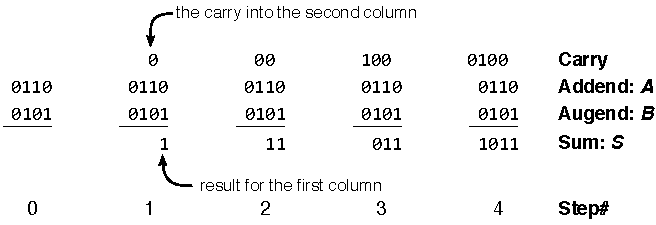
\includegraphics[width=.75\textwidth]{binaryadditionexample2}
  \begin{itemize}\small
    \item The LSB column adds two bits. Every other column adds \alert{three}: $a_i$, $b_i$ and the carry-in $c_i$.
    \item Each column produces a sum $s_i$ and a carry $c_{i+1}$ for the next column.
  \end{itemize}
\end{frame}

\begin{frame}{Half Adder}
  \begin{columns}[c]
  \begin{column}{.45\textwidth}
    \centering\footnotesize\striped
    \begin{tabular}{@{}cc|cc@{}}
      \toprule
      $a_i$ & $b_i$ & $c_{i+1}$ & $s_i$ \\
      \midrule
      0&0&0&0 \\ 0&1&0&1 \\ 1&0&0&1 \\ 1&1&1&0 \\
      \bottomrule
    \end{tabular}\\[3mm]
    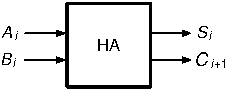
\includegraphics[width=.6\textwidth]{ha_sch}
  \end{column}
  \begin{column}{.53\textwidth}
    \begin{itemize}\small\itemsep3pt
      \item Adds two bits: sum 0 to 2, so two outputs.
      \item It has no carry-in, so it works only at the LSB.
    \end{itemize}
    \[ c_{i+1} = a_ib_i \qquad s_i = a_i \oplus b_i \]
    \centering
    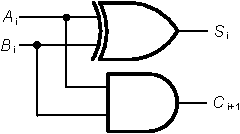
\includegraphics[width=.55\textwidth]{ha_sc}
  \end{column}
  \end{columns}
\end{frame}

\begin{frame}{Full Adder}
  \begin{columns}[c]
  \begin{column}{.5\textwidth}
    \centering\scriptsize\striped
    \begin{tabular}{@{}ccc|cc@{}}
      \toprule
      $a_i$ & $b_i$ & $c_i$ & $c_{i+1}$ & $s_i$ \\
      \midrule
      0&0&0&0&0 \\ 0&0&1&0&1 \\ 0&1&0&0&1 \\ 0&1&1&1&0 \\
      1&0&0&0&1 \\ 1&0&1&1&0 \\ 1&1&0&1&0 \\ 1&1&1&1&1 \\
      \bottomrule
    \end{tabular}\\[2mm]
    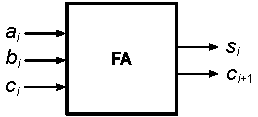
\includegraphics[width=.45\textwidth]{fa_sch}
  \end{column}
  \begin{column}{.48\textwidth}
    \centering
    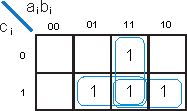
\includegraphics[width=.45\textwidth]{full_adder_map_cout}\hspace{3mm}
    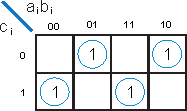
\includegraphics[width=.45\textwidth]{full_adder_map_sum}\\
    {\scriptsize $c_{i+1} = a_ib_i + b_ic_i + a_ic_i$ \hspace{4mm} $s_i = a_i \oplus b_i \oplus c_i$}
    \begin{itemize}\small
      \item Three inputs: the carry-in lets full adders be cascaded.
    \end{itemize}
  \end{column}
  \end{columns}
\end{frame}

\begin{frame}{Full Adder Circuits}
  \centering
  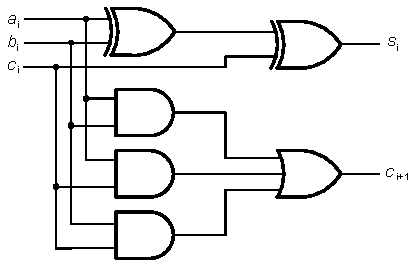
\includegraphics[height=.3\textheight]{full_adder_v1}\hspace{8mm}
  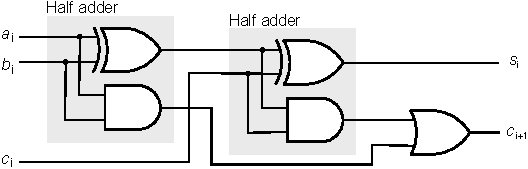
\includegraphics[height=.3\textheight]{full_adder_v2}\\[1mm]
  {\small Two-level \hspace{.4\textwidth} Multi-level}
  \begin{itemize}\small\itemsep2pt
    \item Multi-level: $c_{i+1} = a_ib_i + (a_i \oplus b_i)c_i$. It is faster when full adders are cascaded.
    \item $(a_i \oplus b_i)c_i$ may replace $(a_i + b_i)c_i$: when $a_i = b_i = 1$ the other term $a_ib_i$ already forces $c_{i+1} = 1$.
  \end{itemize}
\end{frame}

%===============================================================================
\section{Ripple Carry Adders}
%===============================================================================

\begin{frame}{Ripple-Carry Adder}
  \begin{columns}[c]
  \begin{column}{.3\textwidth}
    \centering
    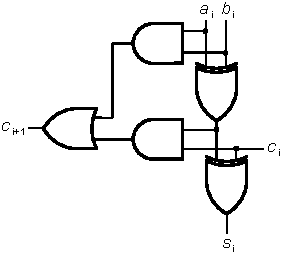
\includegraphics[width=.7\textwidth]{full_adder_v5}\\
    {\scriptsize Cascadable full adder}\\[2mm]
    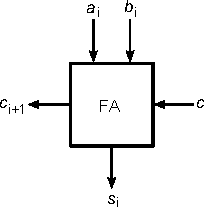
\includegraphics[width=.5\textwidth]{fasym_v2}
  \end{column}
  \begin{column}{.68\textwidth}
    \centering
    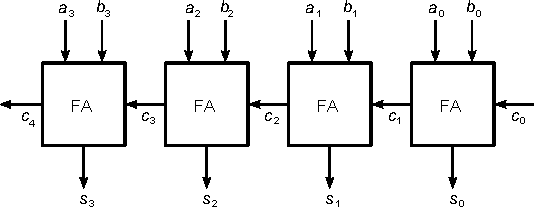
\includegraphics[width=\textwidth]{rca4}
    \begin{itemize}\small\itemsep2pt
      \item $n$ full adders in sequence; stage 0 has $c_0 = 0$ (a half adder would also work, but full adders keep the design uniform).
      \item The carry ripples from stage to stage, so each adder waits for the previous one.
      \item Simple and cheap, but slow: fine where speed is not critical.
    \end{itemize}
  \end{column}
  \end{columns}
\end{frame}

\begin{frame}{Subtraction with an Adder}
  \begin{columns}[c]
  \begin{column}{.4\textwidth}
    \centering
    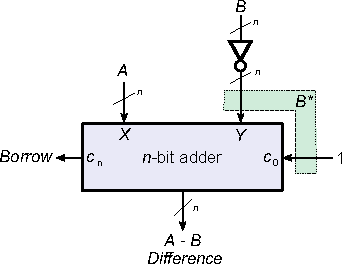
\includegraphics[width=.9\textwidth]{subbyadd}
  \end{column}
  \begin{column}{.58\textwidth}
    \begin{itemize}\small\itemsep3pt
      \item Invert the $B$ inputs and set the carry-in to 1:
    \end{itemize}
    \[ S = A + \overline{B} + 1 = A + B^* = A + (2^n - B) = A - B + 2^n \]
    \begin{itemize}\small\itemsep3pt
      \item The extra $2^n$ is the discarded carry, so $S = A - B$.
      \item Works with any adder: no dedicated subtractor circuit is needed.
    \end{itemize}
  \end{column}
  \end{columns}
\end{frame}

%===============================================================================
\section{Delay Analysis}
%===============================================================================

\begin{frame}{Critical Path}
  \begin{columns}[c]
  \begin{column}{.5\textwidth}
    \begin{itemize}\small\itemsep3pt
      \item The \alert{critical path} is the path with the longest delay. It sets the circuit's maximum speed.
      \item Model: $\tau$ = delay of one gate; XOR = $2\tau$, other gates $\tau$.
    \end{itemize}
    \centering
    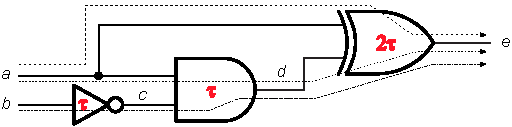
\includegraphics[width=.9\textwidth]{criticalpath}
  \end{column}
  \begin{column}{.48\textwidth}
    \centering\small\striped
    \begin{tabular}{@{}lc@{}}
      \toprule
      \textbf{Path} & \textbf{Delay} \\
      \midrule
      $a \to e$ & $2\tau$ \\
      $a \to d \to e$ & $3\tau$ \\
      $b \to c \to d \to e$ & $4\tau$ \\
      \bottomrule
    \end{tabular}\\[2mm]
    {\small Critical path delay: $4\tau$.}
  \end{column}
  \end{columns}
\end{frame}

\begin{frame}{Delay of a Ripple-Carry Adder}
  \begin{columns}[c]
  \begin{column}{.4\textwidth}
    \centering
    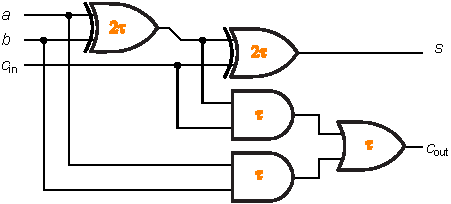
\includegraphics[width=.9\textwidth]{full_adder_v4a}
    \begin{itemize}\scriptsize
      \item $a_i, b_i \to c_{i+1}$: $4\tau$
      \item $a_i, b_i \to s_i$: $4\tau$
      \item $c_i \to c_{i+1}$: $2\tau$
      \item $c_i \to s_i$: $2\tau$
    \end{itemize}
  \end{column}
  \begin{column}{.58\textwidth}
    \centering
    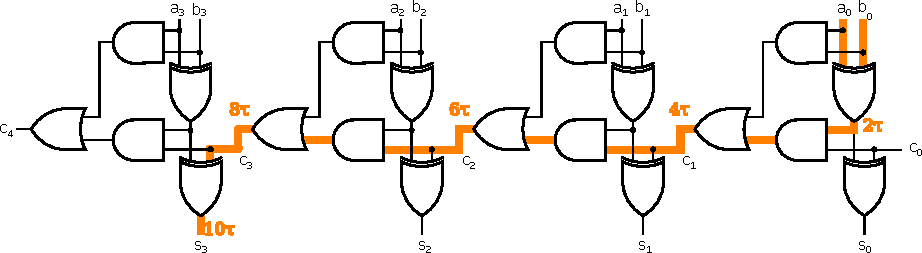
\includegraphics[width=\textwidth]{rcaanalysis}
    \small The critical path runs from $a_0/b_0$ to $s_{n-1}$: $4\tau$ for the first carry, $2\tau$ for each of $n-2$ middle stages, $2\tau$ for the last sum.
    \[ t_{pd} = [4 + 2(n-2) + 2]\tau = (2n + 2)\tau \]
  \end{column}
  \end{columns}
\end{frame}

\begin{frame}{Back to the Opening Question}
  \begin{block}{How slow is a 64-bit ripple adder?}
    \small $t_{pd} = (2n + 2)\tau$. For $n = 64$: $130\tau$, about seven times the $18\tau$ of an 8-bit adder (a 16-bit adder takes $34\tau$).\\[2mm]
    The delay grows \alert{linearly} with $n$. To fix it, we must speed up the carry chain. Three well-known techniques are carry look-ahead, carry-select and carry-save; this chapter covers carry look-ahead.
  \end{block}
\end{frame}

%===============================================================================
\section{Carry Look-Ahead Adders}
%===============================================================================

\begin{frame}{Generate and Propagate}
  \begin{columns}[c]
  \begin{column}{.5\textwidth}
    \begin{itemize}\small\itemsep3pt
      \item A CLA computes $c_{i+1}$ \emph{without waiting} for $c_i$, using a two-level circuit.
      \item Carry-out is 1 when $a_i = b_i = 1$ (\alert{generate}), or when one input is 1 and the carry-in is 1 (\alert{propagate}).
    \end{itemize}
    \[ g_i = a_ib_i \qquad p_i = a_i + b_i \]
    \[ c_{i+1} = g_i + p_ic_i \]
  \end{column}
  \begin{column}{.48\textwidth}
    \centering\scriptsize\striped
    \begin{tabular}{@{}ccc|c|cc@{}}
      \toprule
      $a_i$ & $b_i$ & $c_i$ & $c_{i+1}$ & $g_i$ & $p_i$ \\
      \midrule
      \multicolumn{6}{l}{\textit{Carry kill}} \\
      0&0&0&0&0&0 \\ 0&0&1&0&0&0 \\
      \multicolumn{6}{l}{\textit{Carry propagate}} \\
      0&1&0&0&0&1 \\ 0&1&1&1&0&1 \\ 1&0&0&0&0&1 \\ 1&0&1&1&0&1 \\
      \multicolumn{6}{l}{\textit{Carry generate}} \\
      1&1&0&1&1&1 \\ 1&1&1&1&1&1 \\
      \bottomrule
    \end{tabular}
  \end{column}
  \end{columns}
\end{frame}

\begin{frame}{Look-Ahead Carry Equations}
  \begin{columns}[c]
  \begin{column}{.55\textwidth}
    \small
    \begin{align*}
      c_1 &= g_0 + p_0c_0 \\
      c_2 &= g_1 + p_1g_0 + p_1p_0c_0 \\
      c_3 &= g_2 + p_2g_1 + p_2p_1g_0 + p_2p_1p_0c_0 \\
      c_4 &= g_3 + p_3g_2 + p_3p_2g_1 + p_3p_2p_1g_0 \\
          &\quad + p_3p_2p_1p_0c_0
    \end{align*}
    Each $c_i$ depends only on $c_0$, not on $c_{i-1}$.
  \end{column}
  \begin{column}{.43\textwidth}
    \centering
    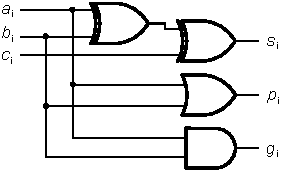
\includegraphics[width=.8\textwidth]{pfaschv3}\\
    {\scriptsize Partial full adder (PFA): $s_i$, $p_i$, $g_i$}
  \end{column}
  \end{columns}
\end{frame}

\begin{frame}{4-Bit Carry Look-Ahead Adder}
  \begin{columns}[c]
  \begin{column}{.5\textwidth}
    \centering
    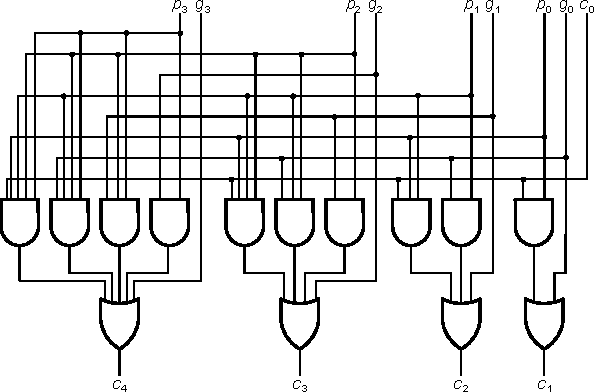
\includegraphics[width=.9\textwidth]{clg}\\
    {\scriptsize Carry look-ahead generator}
  \end{column}
  \begin{column}{.48\textwidth}
    \centering
    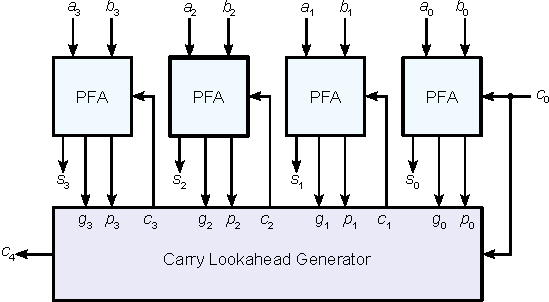
\includegraphics[width=.9\textwidth]{cla-v1}\\
    {\scriptsize One generator and four partial full adders}
  \end{column}
  \end{columns}
  \small
  \[ t_{pd,\mathrm{CLA4}} = [1 + 2 + 2]\tau = 5\tau \]
  {\footnotesize $1\tau$ for $p_i, g_i$; $2\tau$ for $c_4$ from $c_0$; $2\tau$ for $s_3$ from $c_3$.}
\end{frame}

\begin{frame}{Cascading CLA Blocks}
  \centering
  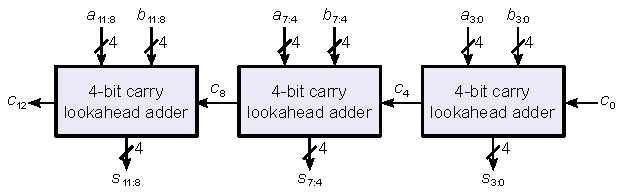
\includegraphics[width=.75\textwidth]{cla12}
  \begin{itemize}\small\itemsep3pt
    \item A single CLA is very fast but needs much hardware, especially beyond 4 bits. Larger adders cascade CLA4 blocks.
    \item With $m$ blocks: $t_{pd} = [1 + 2m + 2]\tau = (2m + 3)\tau$.
    \item 12 bits (3 blocks): $9\tau$, versus $26\tau$ for a 12-bit ripple adder.
  \end{itemize}
\end{frame}

%===============================================================================
\section{Comparators}
%===============================================================================

\begin{frame}{Digital Comparators}
  \begin{columns}[c]
  \begin{column}{.5\textwidth}
    \begin{itemize}\small\itemsep3pt
      \item Compare the MSBs first. If they differ, stop; if equal, move to the next bit.
      \item \alert{Equality} comparators: output when two words are equal (e.g.\ a security lock).
      \item \alert{Magnitude} comparators: $A<B$, $A=B$, $A>B$.
      \item Comparator ICs for 4 and 8 bits can be cascaded for bigger words.
    \end{itemize}
  \end{column}
  \begin{column}{.48\textwidth}
    \centering\small\striped
    \begin{tabular}{@{}cc|ccc@{}}
      \toprule
      $A$ & $B$ & $L$ & $E$ & $G$ \\
      \midrule
      0&0&0&1&0 \\ 0&1&1&0&0 \\ 1&0&0&0&1 \\ 1&1&0&1&0 \\
      \bottomrule
    \end{tabular}\\[2mm]
    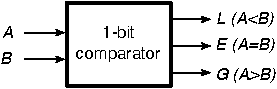
\includegraphics[width=.7\textwidth]{1bitcomp_sch}\\[1mm]
    {\small $L = \overline{A}B$, $\ E = \overline{A\oplus B}$, $\ G = A\overline{B}$}
  \end{column}
  \end{columns}
\end{frame}

%===============================================================================
\section{Parity}
%===============================================================================

\begin{frame}{Parity Generator}
  \begin{columns}[c]
  \begin{column}{.5\textwidth}
    \begin{itemize}\small\itemsep3pt
      \item Parity detects single-bit errors. \alert{Even parity}: the number of 1s in data plus parity bit is even.
      \item $P = D_7 \oplus D_6 \oplus \cdots \oplus D_0$: $P = 1$ when the data has an odd number of 1s.
      \item `a' = 1100001 has three 1s, so $P = 1$; codeword 11100001.
    \end{itemize}
  \end{column}
  \begin{column}{.48\textwidth}
    \centering
    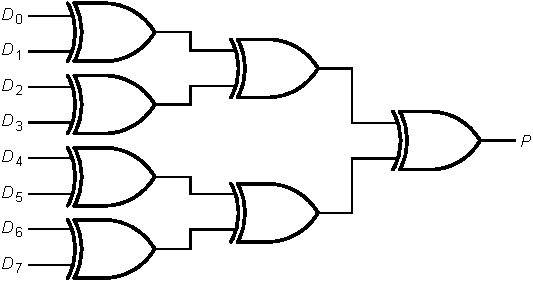
\includegraphics[width=\textwidth]{paritynetwork}
  \end{column}
  \end{columns}
\end{frame}

\begin{frame}{Parity Checker}
  \begin{columns}[c]
  \begin{column}{.55\textwidth}
    \centering
    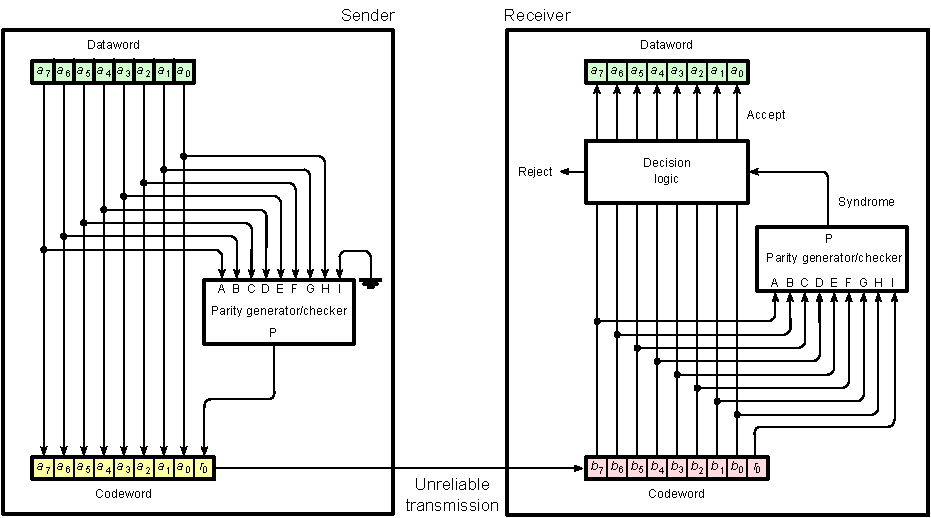
\includegraphics[width=\textwidth]{parity8send}
  \end{column}
  \begin{column}{.43\textwidth}
    \begin{itemize}\small\itemsep4pt
      \item The receiver computes the \alert{syndrome} $S = P \oplus D_7 \oplus \cdots \oplus D_0$.
      \item $S = 0$: no error detected. $S = 1$: reject the byte. Changing 11100001 to 11100000 gives $S = 1$.
      \item An even number of bit errors is not detected, and parity cannot correct errors.
    \end{itemize}
  \end{column}
  \end{columns}
\end{frame}

%===============================================================================
\section{Summary}
%===============================================================================

\begin{frame}{Summary}
  \begin{itemize}\itemsep3pt\small
    \item A \alert{half adder} adds two bits; a \alert{full adder} also takes a carry-in. Full adders chain into an $n$-bit \alert{ripple-carry adder}.
    \item Ripple-carry delay grows linearly with $n$; \alert{carry look-ahead} shortens the carry chain with generate and propagate signals.
    \item \alert{Signed overflow}: $V = c_{n-1} \oplus c_n$. Carry out alone is not an overflow indicator for two's complement.
    \item \alert{Two's-complement subtraction}: add the inverted operand with carry-in 1, so one adder does both.
    \item A \alert{magnitude comparator} gives $A<B$, $A=B$, $A>B$ by comparing from the most significant end.
    \item Parity bits detect single-bit errors but cannot correct them.
  \end{itemize}
  \begin{block}{Looking ahead}
    Chapter 10 adds the missing ingredient, \emph{memory}, with latches and flip-flops.
  \end{block}
\end{frame}

\end{document}
